\documentclass[iop,apj]{emulateapj}

\usepackage{subfigure}
%\documentclass{aastex}
\usepackage{natbib}
\usepackage{amsmath,amssymb}
%\usepackage{apjfonts}
%\usepackage{xspace}
%\usepackage{rotating}
%\usepackage[max]{morefloats}
%\usepackage[usenames]{color}
%\usepackage{color}
\usepackage{graphicx}

\newcommand{\cm}{\textbf}

\usepackage[plainpages=false, colorlinks=true, anchorcolor=blue, linkcolor=blue, citecolor=blue, bookmarks=false]{hyperref}
\citestyle{apj}


\shorttitle{Pulsar distances from GAIA}
\def\beq{\begin{equation}}
\def\eeq{\end{equation}}
\def\bi{\begin{itemize}}
\def\ei{\end{itemize}}
\def\ben{\begin{enumerate}}
\def\een{\end{enumerate}}
\def\bea{\begin{eqnarray}}
\def\eea{\end{eqnarray}}


\newcommand{\tgw}{t_\mathrm{gw}}
\newcommand{\fgw}{f_\mathrm{gw}}
\newcommand{\thard}{t_\mathrm{h}}


\begin{document}

\title{Parallax Distance Measurements to seven binary Millisecond Pulsars from GAIA DR2}
 
\author{
Chiara~M.~F.~Mingarelli\altaffilmark{1, $\dagger$} , 
Lauren Anderson\altaffilmark{1},
Megan Bedell\altaffilmark{1},
David N. Spergel\altaffilmark{1,2}
}

\altaffiltext{$\dagger$}{cmingarelli@flatironinstitute.org}
\affil{$^{1}$ Center for Computational Astrophysics, Flatiron Institute, 162 5th Ave, New York, NY 10010, USA}
\affil{$^{2}$ Department of Astrophysical Sciences, Princeton University, Peyton Hall, Princeton, NJ 08544-0010, USA}


\begin{abstract}
We report parallax distance measurements to seven binary millisecond pulsars -- white dwarf systems: J0437-4715, J1012+5307, J1024-0719, J1804-2717, J1910+1256, J1955+2908 and J2033+1734, using GAIA DR2 data. The distance measurements from GAIA DR2 are to the white dwarfs, and are [[CONSISTENT/INCONSISTENT]] with dispersion measure estimates from current galactic electron density models. We compare the GAIA DR2 distance measurements to other reported parallax distance measurements where available and find them to be [[CONSISTENT/INCONSISTENT]]. We also report the electron number density in the direction of pulsars J1804-2717, J1955+2908, J2033+1734, which can be used to update galactic electron density models.
\end{abstract}

\keywords{
Gravitational waves --
Pulsars:~general --
White Dwarfs:~general --
}

\section{Introduction}
\label{sec:intro}
Millisecond pulsars (MSPs) are some of the best clocks in nature~\citep{bkh+82}, and as such, are used in a wide variety of physics experiments ranging from test of dark matter to gravitational-wave (GW) detection. Due to their formation history, MSPs are often found in binary systems...

When parallax distance measurements are not available, distances to MSPs are estimated via their Dispersion Measure (DM) -- a frequency-dependent delay in the pulse arrival time, due to the radio waves traveling through the ionized interstellar medium of the galaxy, see e.g.~\citep{pulsarAstronomy}. This delay is proportional to the product of the mean electron number density, $\langle n_e \rangle$, and the distance to the pulsar, $D$. One must therefore have a handle on the galactic distribution of electrons in order to compute the pulsar distances. Such models have been proposed by~\cite{cl02,cl03, ymw+17}, among others, however, since the relationship between DM and pulsar distances can only be calibrated by pulsars with known distances (measured by e.g. timing parallax), there are large errors associated with these inferred distance measurements, of the order of 20\%.

Precise pulsar distance measurements are important for a variety of reasons, but in particular for pulsar timing array (PTA) experiments~\cite{abb+17}, which aim to detect nanohertz GWs from both individual inspiralling supermassive black hole binaries (SMBHBs), and the GW background (GWB) from the cosmic merger history of these SMBHBs. In particular, precise pulsar distance measurements can improve the sensitivity of PTAs to continuous GW sources (from individual SMBHB systems)~\citep{zwx+16}  including measuring the evolution of supermassive black hole binaries with pulsar timing arrays~\cite{mgs+12}.

\section{Results}
Using IPTA DR1~\citep{v+16}, we cross-referenced the MSP locations with objects in GAIA DR1~\citep{gaiaDR1}, updating the pulsar positions to the GAIA epoch, and searching around the pulsar position within 3 arcseconds. 

We report parallax distance measurements to pulsars J0437-4715, J1012+5307, J1024-0719, J1804-2717, J1910+1256, J1955+2908 and J2033+1734, using GAIA DR2 data. Of these, J1804-2717, J1955+2908, J2033+1734 had previously unknown parallax measurements. With these measurements, and together with the dispersion measure from pulsar timing experiments, we can now report the electron number density in the line-of-sight to these pulsars for the first time,
\beq
n_e = \frac{DM}{D}\, ,
\eeq
where $DM$ is the dispersion measure, and $D$ is the distance to the object -- in this case the binary pulsar system. These three new measurements can in turn be used to update the galactic electron density model~\cite{cl02,cl03, ymw+17}
\begin{table*}[h]
\begin{center}
\caption{\label{tab:results} Summary of results. *1024 has several issues with its distance measurement which we should discuss. We can also compare distance measurements between the Yao et al. 2017 model and the more famous NE 2001 model. Dispersion measures were reported in \cite{v+16} and references therein, and pulsar distances were calculated based on this DM via the online tools for NE 2001 and YMW16. $ ^\dagger$We assume the error in the distance from the YMW 16 model is $\pm 20\%$. }
\begin{tabular}{@{\;\;}l@{\;\;}l@{\;}l@{\;}l@{\;}l@{\;}l@{\;}l@{\;}l@{\;}c@{\;}}
\hline\hline
Pulsar 		& DM (cm$^{-3}$pc)	& $D_{DM}$ (pc) & $D_{DM}$ (pc) & $D_\pi$ (pc) & $D_\pi$ (pc) & $\mu_P$ (mas/yr) 	& $\mu_G$ (mas/yr)& Ref\\
			&			&NE 2001 	&YMW 16$ ^\dagger$		& Parallax			& GAIA		& Pulsar & GAIA\\
\hline
 J0437-4715 	& 2.64  & $139^{+33}_{-29}$ & 156.1 &is $156.3^{+1.3}_{-1.3}$ 	& TBD		&	141.29 $\pm$ 0.06 	&  TBD 	&	\cite{v+16, dvt+08, dcl+16}\\
 J1012+5307 	& 9.02	& $411^{+59}_{-56}$	& 804.5 		& $1150^{+240}_{-240}$		&TBD			&	25.615 $\pm$ 0.010	&		& 	\cite{v+16, dcl+16}\\
 J1024-0719* 	& 6.49	& $386^{+39}_{-38}$	&	382.3	& $1300^{+600}_{-300}$		&TBD			&	59.72 $\pm$ 0.06	&		& 	\cite{v+16, kkn+16, dcl+16}\\
 J1804-2717 	& 24.67	&  	$776^{+102}_{-108}$	& 800.5 		& -							&TBD			&	17.3 $\pm$ 2.4		&		& 	\cite{v+16, dcl+16}\\
 J1910+1256 	& 38.06	& $2327^{+311}_{-317}$	&1496.0 		& $550^{+460}_{-460}$		&TBD			&	7.37 $\pm$ 0.15		&		&	\cite{v+16, dcl+16}\\
 J1955+2908 	&104.58	&  $4644^{+577}_{-553}$		&	6306.2 	& -							&TBD			&	4.75 $\pm$ 0.26		& 		&	\cite{v+16, dcl+16}\\
 J2033+1734 	& 25.20	& $2004^{+175}_{-266}$ 	&	1747.7 	& -							&TBD			&	10.8 $\pm$ 0.7		&		& 	\cite{v+16, dcl+16}\\
 \hline \hline
 \end{tabular}
\end{center}
\end{table*}
%
We discarded white dwarfs associated with J0613-0200 and (J1804-2717???) since the resultant luminosities of the objects associated with these pulsars are too bright to be WDs, with mean photo $g$ magnitudes of 15.47 and 16.19. Indeed, the star in the line of sight to J0613-0200 was previously reported by XX.


\begin{figure*}
\centering
    \begin{subfigure}
        \centering
        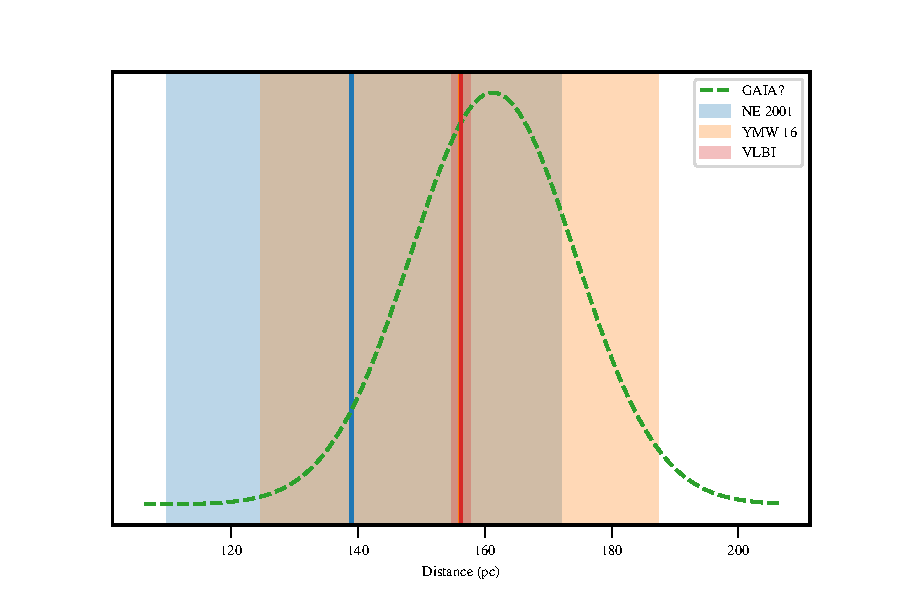
\includegraphics[scale=.5]{../figures/J0437_distances.pdf}
        \caption{}\label{fig:fig_a}
    \end{subfigure} %

    \begin{subfigure}
        \centering
        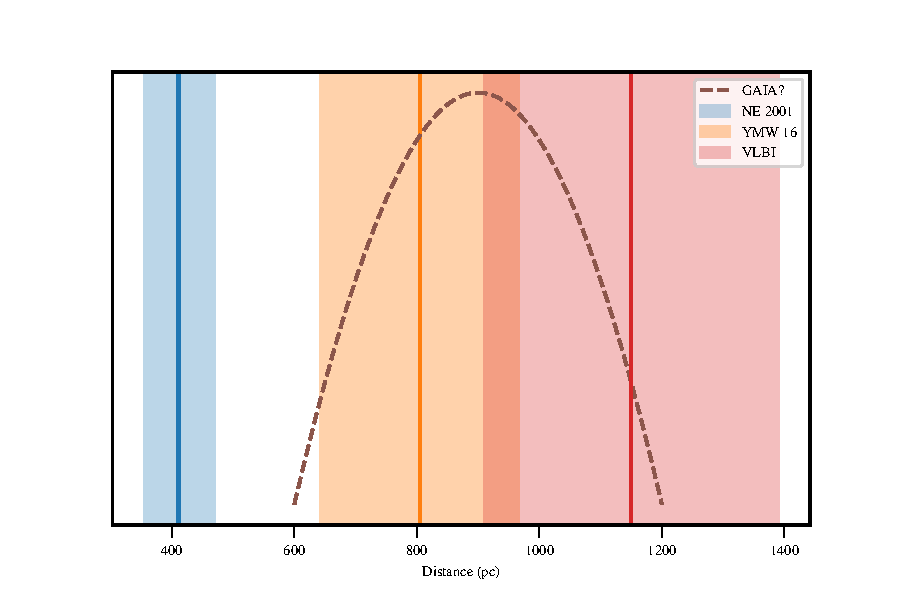
\includegraphics[scale=.5]{../figures/J1012_distances.pdf}
        \caption{}\label{fig:fig_b}
    \end{subfigure} %
    
    \begin{subfigure}
        \centering
        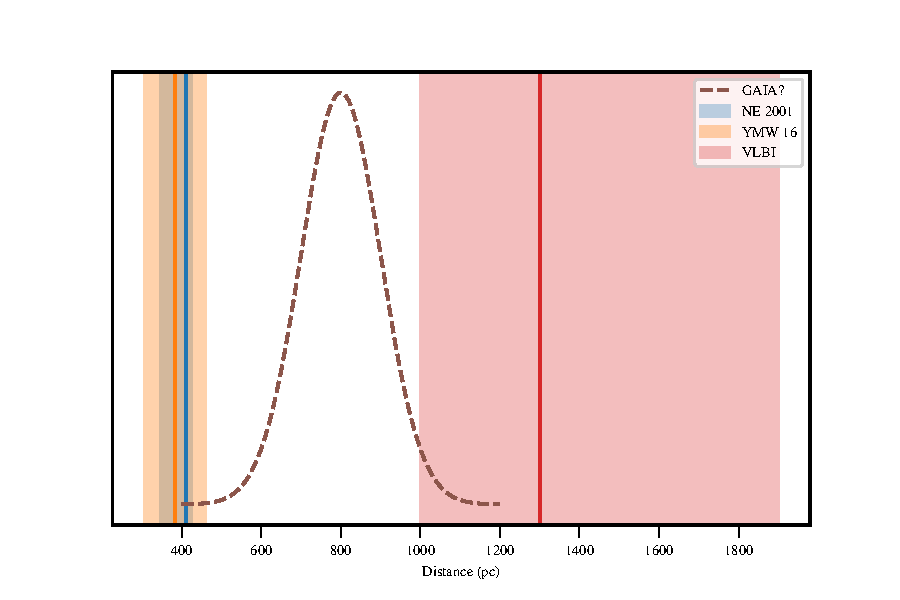
\includegraphics[scale=.5]{../figures/J1024_distances.pdf}
        \caption{}\label{fig:fig_c}
    \end{subfigure}
\caption{these are placeholders}
\end{figure*}

\section{Discussion}



\acknowledgements

\emph{Acknowledgments.}
The authors thank Yuri Levin, Adrian Price-Whelan, Stephen Feeney (and likely others) for useful conversations.




\bibliographystyle{apj}
\bibliography{apjjabb,bib}


\end{document}





